\documentclass{beamer} %

%%%BASICS
\usepackage[utf8]{inputenc}
\usepackage{csquotes}
\usepackage{enumerate}
\usepackage{mathtools}
\usepackage{tikz}
\usepackage{tikz-qtree}
\usetikzlibrary{trees}
\usepackage{amsfonts}
\usepackage{hyperref}

\usepackage{multicol}
\usepackage{graphicx}
\usepackage{epigraph}

\renewcommand{\epigraphflush}{center}
\renewcommand{\epigraphwidth}{300}


%%%Commandes

\newcommand{\N}{\mathbb{N}}
\newcommand{\Q}{\mathbb{Q}}

%%%START THEME SETTINGS
\usetheme{CambridgeUS}
\usecolortheme{beaver}
\usefonttheme{professionalfonts}
\setbeamertemplate{itemize item}{\color{black} $\blacksquare$}
%%%END THEME SETTINGS

%%%START APA
\usepackage[british]{babel}
\usepackage[backend=biber,style=apa]{biblatex}
\DeclareLanguageMapping{british}{british-apa}
\addbibresource{references.bib}
%% APA citing
%% \cite{t} - Uthor und Richter, 2010
%% \textcite{t} - Uthor und Riter (2010)
%% \parencite{t} - (Uthor & Riter, 2010)
%% \parencite[Chapt.~4]{t} - (Uthor & Riter, 2010, S. 15)
%%%END APA


\title[Arithmetic and Set Theory]{Foundations of Mathematics: On the Translations Between 
Arithmetic and Set Theory}
\institute[COLABS]{COLABS Tohoku University \and UCLouvain}
\author{Thibaut Kouptchinsky}

\date{February 2023}

\begin{document}

\begin{frame}
	\titlepage;
\end{frame}

\begin{frame}{\textbf{The main question}: What are the appropriate axioms to prove the theorems of mathematics }

        \epigraph{\textit{Fondations of mathematics is the study of the most basic concepts 
        and logical structure of mathematics, with an eye to the unity of human knowledge}}{\textit{Stephen G. Simpson \\ SSOA (second edition)}}
\pause Aristote, Euclide, Descartes, Cauchy, Weierstraß, Dedekind, Peano, Frege, Russell, 
Cantor, Hilbert, Brouwer, Weyl, von Neumann, Skolem, Tarski, Heyting, Gödel, $\dots$
\end{frame}

\begin{frame}{The Set Theory of Zermelo and Fraënkel}
    \begin{example}
         \begin{enumerate}
            \item<1-> The set of natural numbers: $\mathbb{N} = \{0, 1, 2, 3, \dots, 2^{82,589,933}-1, \dots \}$.
            \item<2-> The graph of the function $\sin \colon \mathbb{R} \to \mathbb{R}$: $\{(x,\sin(x)) : x \in \mathbb{R}\}$.
        \end{enumerate}
    \end{example}
    \pause 
    \pause 
    A counter-example, the Russel's Paradox: \begin{align*}
        S = \{ X : X \not\in X\}
    \end{align*}
    \begin{itemize}
        \item<5-> If $S \in S$, then $S \not\in S$;
        \item<6-> If $S \not\in S$, then $S \in S$. 
    \end{itemize}
\end{frame}

\begin{frame}{The axioms of $\mathsf{ZF}$}
    \begin{enumerate}
        \item<1-> There exists a set and this set is empty; $\emptyset$.
        \item<2-> \textsc{Pair}: If $a$ and $b$ are sets, we can form $\{a,b\}$.
        \item<3-> \textsc{Separation}: If $P$ is property and $X$ is a set, we can form \begin{align*}
            \{u \in X \mid P(u)\}.    
        \end{align*}
        \item<4-> \textsc{Infinity}: There exists an infinite set.
        \item<5-> plus $5$ others $\dots$ 
    \end{enumerate}
\end{frame}

\begin{frame}{The Von Neumann construction of $\mathbb{N}$}
    \begin{align*}
        &0 = \{ \ \} &&= \emptyset,
        \\&1 = \{ 0 \} &&=\{\emptyset\}
        \\&2 = \{ 0, 1 \} &&=\{ \emptyset, \{\emptyset\} \}
        \\&3 = \{ 0, 1, 2\} &&=\{ \emptyset, \{\emptyset\}, \{ \emptyset, \{\emptyset\} \}\}
        \\&\dots
        \\&n + 1 = n \cup \{ n\} &&=\{0,1,2, \dots , n\}
        \\&\dots
    \end{align*}
\end{frame}

\begin{frame}
    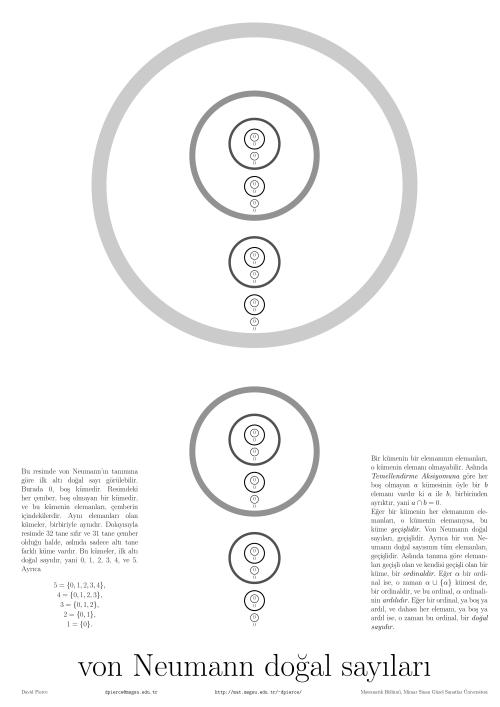
\includegraphics[width=\textwidth]{ordinaller-poster-small.jpg}
\end{frame}

\begin{frame}{The Realm of Second-order Arithmetic}
    Friedman and Simpson: Encoding the ordinary mathematics with only 
    \begin{enumerate}
        \item Natural numbers $n \in \mathbb{N}$;
        \item Sets of natural numbers $S \subseteq \mathbb{N}$.
    \end{enumerate}
    \pause
    Example: $\mathbb{Z} \times \mathbb{Z}$ is countable
    \begin{figure}
        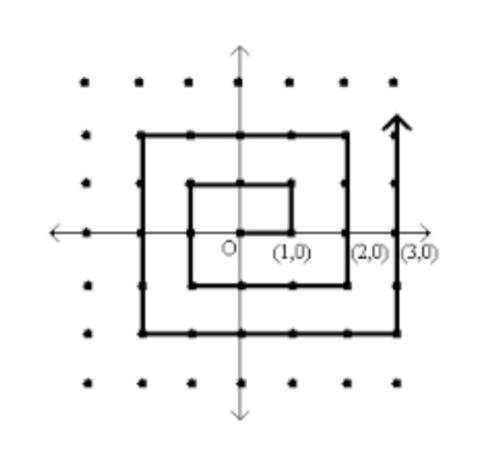
\includegraphics[width=5cm]{IMG_0607.jpg}
    \end{figure}
    
\end{frame}

\begin{frame}{(Well-founded) Trees}
    \begin{definition}
        A tree is a subset of finite sequences of natural numbers ($T \subseteq \mathbb{N}^{<\infty}$), such that 
        leafs are the biggest sequences and root is the empty sequence. Moreover there is a branch in $T$ from the root 
        to any leaf.
    \end{definition}
    \pause
    \begin{figure}
        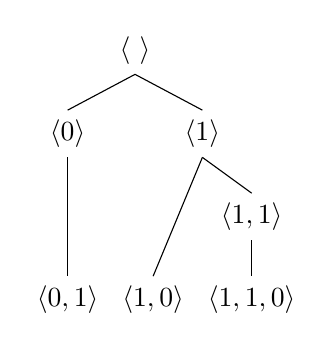
\begin{tikzpicture}
            \tikzset{frontier/.style={distance from root=90pt}}
                \Tree [.{$\langle \ \rangle$}
                [.{$\langle 0 \rangle$} {$\langle 0, 1 \rangle$} ]
                [.\node(a){$\langle 1 \rangle$}; {$\langle 1, 0 \rangle$} 
                [.{$\langle 1, 1 \rangle$} {$\langle 1, 1, 0 \rangle$} ] ]]
        \end{tikzpicture}
    \end{figure}
\end{frame}

\begin{frame}{Another example of tree}
    \begin{figure}
        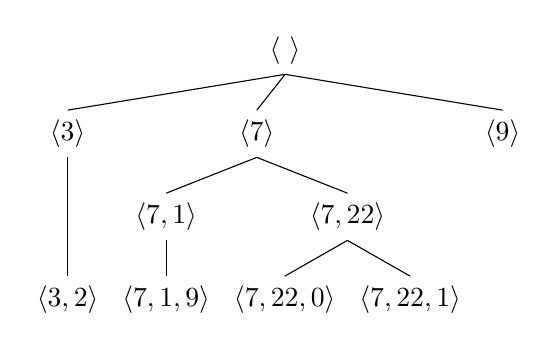
\begin{tikzpicture}
            \tikzset{frontier/.style={distance from root=90pt}}
                \Tree [.{$\langle \ \rangle$}
                [.{$\langle 3 \rangle$} {$\langle 3, 2 \rangle$} ]
                [.{$\langle 7 \rangle$} 
                [.{$\langle 7, 1 \rangle$} {$\langle 7, 1, 9 \rangle$} ]
                [.{$\langle 7, 22 \rangle$} {$\langle 7, 22, 0\rangle$} {$\langle 7, 22, 1\rangle$} ] ]
                [.{$\langle 9 \rangle$} ] ]
        \end{tikzpicture}
    \end{figure}    
\end{frame}

\begin{frame}{Set Theory in Second Order Arithmetic}
    We encode a set by a tree $T$ where \begin{enumerate}
        \item<2-> If $\sigma \in T$ is a leaf, then $|\sigma|$ code the emptyset,
        \item<3-> If $\tau$ is deeper than $\sigma$ on a branch, then it code $|\tau| \in |\sigma|$.
    \end{enumerate}
    \pause 
    \pause
    \pause
    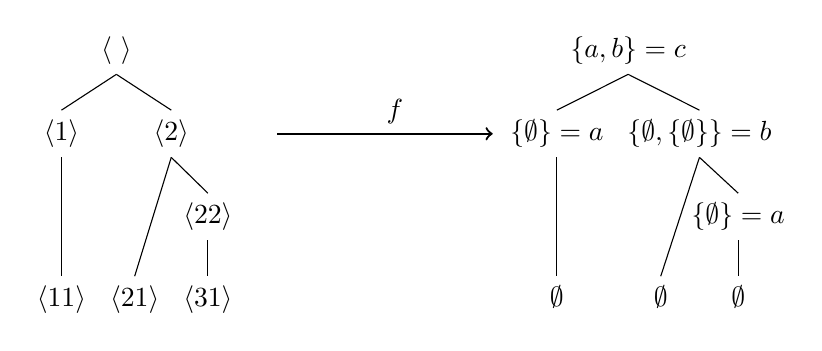
\begin{tikzpicture}
            \tikzset{frontier/.style={distance from root=90pt}}
            
                
                \begin{scope}
                    \Tree [.{$\langle \ \rangle$}
                    [.{$\langle 1 \rangle$} {$\langle 11 \rangle$} ]
                    [.\node(a){$\langle 2 \rangle$}; {$\langle 21 \rangle$} 
                    [.{$\langle 22 \rangle$} {$\langle 31 \rangle$} ] ]]
                \end{scope} 
                
                \begin{scope}[xshift=6.5cm]
                    \Tree [.{$\{a,b\} = c$}
                    [.\node(b){$\{\emptyset\}=a$}; {$\emptyset$} ]
                    [.{$\{\emptyset, \{\emptyset\}\}=b$} {$\emptyset$} 
                    [.{$\{\emptyset\}=a$} {$\emptyset$} ] ]]     
                \end{scope}
                \draw[thick, ->, shorten <=1cm, shorten >= 0.1cm ] (a)--(b) node[pos=0.65pt, above] {$f$};
    
    \end{tikzpicture}
\end{frame}

\end{document}
